\section{Durchführung}
\label{sec:Durchführung}
In diesem Versuch werden zunächst Acrylzylinder einmal mit dem Durchschallungs-
und einmal mit dem Impuls-Echo-Verfahren vermessen. Hierzu werden für x Zylinder
die Schalllaufzeiten aufgezeichnet. Beim Impuls-Echo-Verfahren werden zusätzlich
die Amplituden der Impulse gemessen, um den exponentiellen Abfall dieser
nachzuweisen, wobei eine feste Verstärkung des Signales (engl. gain), sowie eine
zeitlich variable Verstärkung (engl. time gain control, kurz TGC) zur Verfügung
stehen, um die Signale zu verdeutlichen. Da beim Impuls-Echo-Verfahren die
Acrylzylinder senkrecht stehen können, um mehr Messdaten zu erhalten, mehrere
Zylinder (mit bidestilliertem Wasser gekoppelt) aufeinander gestellt werden.
Alle Zylinder werden mit Hilfe einer Schieblehre vermessen, um aus ihrer Länge
und der aufgenommenen Laufzeiten die Schallgeschwindigkeit in Acryl zu berechnen.
Nach Bestimmung der Schallgeschwindigkeit werden mit dem Impuls-Echo-Verfahren
Grenzflächen untersucht: zwei dünne Acrylscheiben werden übereinander gekoppelt
und über einen Vorlaufzylinder beschallt. Der Vorlaufzylinder besteht ebenfalls
aus Acryl und sorgt nur dafür, dass die reflektierten Impulse
(welche sehr Schwach ausfallen) gut erkennbar vom ersten Impuls zu unterscheiden
sind.
Abschließend verwendet man das Puls-Echo-Verfahren, um ein Augenmodell \ref{fig:augm} mit
Iris und Linse zu vermessen.
\begin{figure}
  \centering
  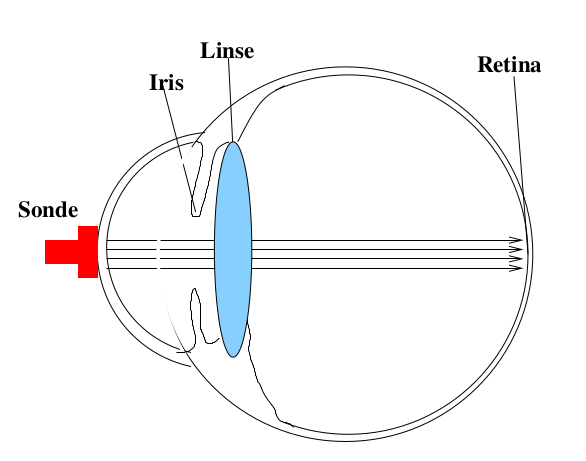
\includegraphics[height=5cm]{logos/Augenmodell.png}
  \caption{Schemtaische Abbildung des Augenmodells}
  \label{fig:augm}
\end{figure}
